\documentclass[12pt]{article}


\usepackage{amsmath}
\usepackage[top=1in, bottom=1in, left=1.25in, right=1.25in]{geometry}
\usepackage{setspace}
\setcounter{secnumdepth}{1}
%\usepackage{tocstyle}
%\usetocstyle{standard}
\renewcommand{\contentsname}{\centerline {\normalsize Table of Contents}}
\usepackage{tocloft}
\renewcommand{\cftsecfont}{\normalsize}
\renewcommand{\cftsecleader}{\cftdotfill{\cftsecdotsep}}
\renewcommand\cftloftitlefont{\normalsize,\bfseries}
\renewcommand\cftlottitlefont{\normalsize,\bfseries}
\usepackage{sectsty}
\sectionfont{\normalsize}
\usepackage{geometry}
\usepackage{pdflscape}
\usepackage{enumitem}
\usepackage{natbib}
\usepackage{mathtools}
\usepackage{dsfont}
\usepackage{bm}
%\usepackage{cite}
\usepackage{float}
\usepackage{placeins}
\usepackage{adjustbox}
\usepackage{lscape}
\usepackage{caption}
%\usepackage{graphicx}	% Including figure files
\usepackage{amsmath}	% Advanced maths commands
\usepackage{amssymb}	% Extra maths symbols
\def\dd#1#2{\frac{d #1}{d #2}}
\def\2dd#1#2{\frac{d^2 #1}{d #2^2}}
\def\pd#1#2{\frac{\partial #1}{\partial #2}}
\def\2pd#1#2{\frac{\partial^2 #1}{\partial #2^2}}
\newcommand\sq{\mbox{\rlap{$\sqcap$}$\sqcup$}}% 
\newcommand\arcdeg{\mbox{$^\circ$}}% 
\newcommand\arcmin{\mbox{$^\prime$}}% 
\newcommand\arcsec{\mbox{$^{\prime\prime}$}}% 
\newcommand\fd{\mbox{$.\!\!^{\mathrm d}$}}% 
\newcommand\fh{\mbox{$.\!\!^{\mathrm h}$}}% 
\newcommand\fm{\mbox{$.\!\!^{\mathrm m}$}}% 
\newcommand\fs{\mbox{$.\!\!^{\mathrm s}$}}% 
\newcommand\diameter{\ooalign{\hfil/\hfil\crcr\mathhexbox20D}}% 
\newcommand\degr{\arcdeg}% 
\newcommand\Sun{\sun}% 
\newcommand\Sol{\sun}% 
\newcommand\sun{\odot}% 
\newcommand\Mercury{\astro{\char1}}% Mercury symbol, "1" 
\newcommand\Venus{\astro{\char2}}% Venus symbol, "2" 
\newcommand\Earth{\earth}% 
\newcommand\Terra{\earth}% 
\newcommand\earth{\oplus}% 
\newcommand\Mars{\astro{\char4}}% Mars symbol, "4" 
\newcommand\Jupiter{\astro{\char5}}% Jupiter symbol, "5" 
\newcommand\Saturn{\astro{\char6}}% Saturn symbol, "6" 
\newcommand\Uranus{\astro{\char7}}% Uranus symbol, "7" 
\newcommand\Neptune{\astro{\char8}}% Neptune symbol, "8" 
\newcommand\Pluto{\astro{\char9}}% Pluo symbol, "9" 
\newcommand\Moon{\astro{\char10}}% Moon symbol, "M" 
\newcommand\Luna{\Moon}% 
\newcommand\Aries{\astro{\char11}}% 
\newcommand\VEq{\Aries}% vernal equinox (Aries) 
\newcommand\Taurus{\astro{\char12}}% 
\newcommand\Gemini{\astro{\char13}}% 
\newcommand\Cancer{\astro{\char14}}% 
\newcommand\Leo{\astro{\char15}}% 
\newcommand\Virgo{\astro{\char16}}% 
\newcommand\Libra{\astro{\char17}}% 
\newcommand\AEq{\Libra}% autumnal equinox (Libra) 
\newcommand\Scorpius{\astro{\char18}}% 
\newcommand\Sagittarius{\astro{\char19}}% 
\newcommand\Capricornus{\astro{\char20}}% 
\newcommand\Aquarius{\astro{\char21}}% 
\newcommand\Pisces{\astro{\char22}}% 
\newcommand\ion[2]{#1$\;${%
\ifx\@currsize\normalsize\small \else
\ifx\@currsize\small\footnotesize \else
\ifx\@currsize\footnotesize\scriptsize \else
\ifx\@currsize\scriptsize\tiny \else
\ifx\@currsize\large\normalsize \else
\ifx\@currsize\Large\large
\fi\fi\fi\fi\fi\fi
\rmfamily\@Roman{#2}}\relax}% 

\newcommand\sbond{\chem@bnd{\@sbnd}}%
\newcommand\dbond{\chem@bnd{\@dbnd}}%
\newcommand\tbond{\chem@bnd{\@tbnd}}%

\graphicspath{{./}{Figures/}}

% Standard journal abbreviations
% Mostly as used by ADS, with a few additions for journals where MNRAS does not
% follow normal IAU style.

\newcommand\aap{A\&A}                % Astronomy and Astrophysics
\let\astap=\aap                          % alternative shortcut
\newcommand\aapr{A\&ARv}             % Astronomy and Astrophysics Review (the)
\newcommand\aaps{A\&AS}              % Astronomy and Astrophysics Supplement Series
\newcommand\actaa{Acta Astron.}      % Acta Astronomica
\newcommand\afz{Afz}                 % Astrofizika
\newcommand\aj{AJ}                   % Astronomical Journal (the)
\newcommand\ao{Appl. Opt.}           % Applied Optics
\let\applopt=\ao                         % alternative shortcut
\newcommand\aplett{Astrophys.~Lett.} % Astrophysics Letters
\newcommand\apj{ApJ}                 % Astrophysical Journal
\newcommand\apjl{ApJ}                % Astrophysical Journal, Letters
\let\apjlett=\apjl                       % alternative shortcut
\newcommand\apjs{ApJS}               % Astrophysical Journal, Supplement
\let\apjsupp=\apjs                       % alternative shortcut
% The following journal does not appear to exist! Disabled.
%\newcommand\apspr{Astrophys.~Space~Phys.~Res.} % Astrophysics Space Physics Research
\newcommand\apss{Ap\&SS}             % Astrophysics and Space Science
\newcommand\araa{ARA\&A}             % Annual Review of Astronomy and Astrophysics
\newcommand\arep{Astron. Rep.}       % Astronomy Reports
\newcommand\aspc{ASP Conf. Ser.}     % ASP Conference Series
\newcommand\azh{Azh}                 % Astronomicheskii Zhurnal
\newcommand\baas{BAAS}               % Bulletin of the American Astronomical Society
\newcommand\bac{Bull. Astron. Inst. Czechoslovakia} % Bulletin of the Astronomical Institutes of Czechoslovakia 
\newcommand\bain{Bull. Astron. Inst. Netherlands} % Bulletin Astronomical Institute of the Netherlands
\newcommand\caa{Chinese Astron. Astrophys.} % Chinese Astronomy and Astrophysics
\newcommand\cjaa{Chinese J.~Astron. Astrophys.} % Chinese Journal of Astronomy and Astrophysics
\newcommand\fcp{Fundamentals Cosmic Phys.}  % Fundamentals of Cosmic Physics
\newcommand\gca{Geochimica Cosmochimica Acta}   % Geochimica Cosmochimica Acta
\newcommand\grl{Geophys. Res. Lett.} % Geophysics Research Letters
\newcommand\iaucirc{IAU~Circ.}       % IAU Cirulars
\newcommand\icarus{Icarus}           % Icarus
\newcommand\japa{J.~Astrophys. Astron.} % Journal of Astrophysics and Astronomy
\newcommand\jcap{J.~Cosmology Astropart. Phys.} % Journal of Cosmology and Astroparticle Physics
\newcommand\jcp{J.~Chem.~Phys.}      % Journal of Chemical Physics
\newcommand\jgr{J.~Geophys.~Res.}    % Journal of Geophysics Research
\newcommand\jqsrt{J.~Quant. Spectrosc. Radiative Transfer} % Journal of Quantitiative Spectroscopy and Radiative Transfer
\newcommand\jrasc{J.~R.~Astron. Soc. Canada} % Journal of the RAS of Canada
\newcommand\memras{Mem.~RAS}         % Memoirs of the RAS
\newcommand\memsai{Mem. Soc. Astron. Italiana} % Memoire della Societa Astronomica Italiana
\newcommand\mnassa{MNASSA}           % Monthly Notes of the Astronomical Society of Southern Africa
\newcommand\mnras{MNRAS}             % Monthly Notices of the Royal Astronomical Society
\newcommand\na{New~Astron.}          % New Astronomy
\newcommand\nar{New~Astron.~Rev.}    % New Astronomy Review
\newcommand\nat{Nature}              % Nature
\newcommand\nphysa{Nuclear Phys.~A}  % Nuclear Physics A
\newcommand\pra{Phys. Rev.~A}        % Physical Review A: General Physics
\newcommand\prb{Phys. Rev.~B}        % Physical Review B: Solid State
\newcommand\prc{Phys. Rev.~C}        % Physical Review C
\newcommand\prd{Phys. Rev.~D}        % Physical Review D
\newcommand\pre{Phys. Rev.~E}        % Physical Review E
\newcommand\prl{Phys. Rev.~Lett.}    % Physical Review Letters
\newcommand\pasa{Publ. Astron. Soc. Australia}  % Publications of the Astronomical Society of Australia
\newcommand\pasp{PASP}               % Publications of the Astronomical Society of the Pacific
\newcommand\pasj{PASJ}               % Publications of the Astronomical Society of Japan
\newcommand\physrep{Phys.~Rep.}      % Physics Reports
\newcommand\physscr{Phys.~Scr.}      % Physica Scripta
\newcommand\planss{Planet. Space~Sci.} % Planetary Space Science
\newcommand\procspie{Proc.~SPIE}     % Proceedings of the Society of Photo-Optical Instrumentation Engineers
\newcommand\rmxaa{Rev. Mex. Astron. Astrofis.} % Revista Mexicana de Astronomia y Astrofisica
\newcommand\qjras{QJRAS}             % Quarterly Journal of the RAS
\newcommand\sci{Science}             % Science
\newcommand\skytel{Sky \& Telesc.}   % Sky and Telescope
\newcommand\solphys{Sol.~Phys.}      % Solar Physics
\newcommand\sovast{Soviet~Ast.}      % Soviet Astronomy (aka Astronomy Reports)
\newcommand\ssr{Space Sci. Rev.}     % Space Science Reviews
\newcommand\zap{Z.~Astrophys.}       % Zeitschrift fuer Astrophysik


\def\av#1{\left\langle #1 \right\rangle}
\def\braket#1#2{\left\langle#1|#1\right\rangle}
\def\opbraket#1#2#3{\left\langle #1\left|#2\right|#3\right\rangle}
\def\ket#1{\left|#1\right\rangle}
\def\cev#1{\reflectbox{\ensuremath{\vec{\reflectbox{\ensuremath{#1}}}}}}

\def\beq{\begin{equation}}
\def\eeq{\end{equation}}
\def\beqs#1\eeqs{\beq\begin{split} #1 \end{split}\eeq}

\usepackage{graphicx}
\graphicspath{{./}{Figures/}}

\usepackage{deluxetable}

%% Units
\def\fm {\,{\tt fm}}
\def\MeV {\,{\tt MeV}}
\def\GeV {\,{\tt GeV}}
\def\degC{\,{^\circ{\tt C}}}
\def\degK{\,{\tt K}}

\usepackage{microtype}
\usepackage[colorlinks=true,backref=false, linktocpage=true,
citecolor=blue,urlcolor=blue,linkcolor=blue,pdfpagemode=UseOutlines]{hyperref}

\hypersetup{%
  bookmarksnumbered=true,
  pdftitle = {Radio Transients: Intermediate to Slow},
  pdfsubject = {Physics},
  pdfauthor = {Sarah I Chastain},
  pdfkeywords = {radio astronomy, transients, Monte-Carlo simulations}
}


\begin{document}
\thispagestyle{empty}
\vspace*{1in}
\begin{center}
\center{Radio Transients: Intermediate to Slow\vspace*{36pt}}
\center{Sarah I Chastain\vspace*{36pt}}
\centerline{M.S. in Physics, May 2021, George Washington Universityl}
\centerline{B.S. in Physics, May 2017 , Univeristy of Memphis}\vspace*{24pt}
\center{A Dissertation submitted to\vspace*{36pt}}
\begin{center}
The Faculty of\\The Columbian College of Arts and Sciences \\ of The George
Washington University\\ in partial fulfillment of the requirements\\ for the degree
of Doctor of Philosophy\\[36pt]
Month Day, Year\\[36pt] %date of degree conferral 
Dissertation directed by\\[\baselineskip]
Dr. Alexander J van der Horst\\
Associate Professor of Physics\\[\baselineskip]
%Name of Co-director\\
%Position
\end{center}
\end{center}
% display page numbers in the footer and centered. Start with roman numerals %
\pagestyle{plain}
\setcounter{page}{1}
\pagenumbering{roman}
\newpage
\begin{doublespace}
\noindent
The Columbian College of Arts and Sciences of The George Washington University certifies that Sarah I Chastain has passed the Final Examination for the degree of Doctor of Philosophy as of \texttt{date of defense}. This is the final and approved form of the dissertation.
\end{doublespace}
\vspace{12pt}
\begin{center}
Radio Transients: Intermediate to Slow

\vspace*{36pt}
Sarah I Chastain
\vspace{24pt}
\end{center}
Dissertation Research Committee:
\vspace{12pt}

\indent Dr. Alexander J van der Horst, Associate Professor of Physics, Dissertation Director
\vspace{12pt}

%\indent Name of Co-director, Position, Dissertation Co-Director
%\vspace{12pt}

\indent Dr. Oleg Kargaltsev , Associate Professor of Physics, Committee Member
\vspace{12pt}

\indent Dr. Bethany Cobb Kung, Associate Professor of Honors and Physics, Committee Member
\vspace{12pt}
%only readers and directors are listed per CCAS. No examiners or chairs.

\newpage
\phantomsection \label{dedication}
\begin{center}
\section*{\textbf{Dedication}}
\end{center}
\addcontentsline{toc}{section}{\textbf{Dedication}}
\begin{center}
\vspace*{6pt}
%\vspace*{-24pt}
%Dedication text goes here.

\end{center}

\doublespacing
\newpage
\phantomsection \label{acknowledgements}
\begin{center}
\section*{Acknowledgments}
\end{center}
\vspace*{6pt}
\addcontentsline{toc}{section}{\textbf{Acknowledgements}}
So long, and thanks for all the fishes.
\doublespacing
\newpage
\begin{center}
\section*{Abstract of Dissertation}
\end{center}
\phantomsection \label{abstract}
\addcontentsline{toc}{section}{\textbf{Abstract of Dissertation}}
\vspace*{-40pt}
\vspace{24pt}
\begin{singlespace}
\center{Radio Transients: Intermediate to Slow}
\end{singlespace}
\vspace{-12pt}
\vspace*{24pt}
Since the beginning of history, humans have looked up to the sky for possible changes and their significance. Transient phenomena, that is, phenomena that appear for a time then disappear, have always been a particular curiousity. Today, we have know a bit more about these phenomena, but they nonetheless continue to be a source of amazing extremes. We know some of these to be collapsing neutron stars, neutron stars with extremely high magnetic field strength, matter accreting on to black holes, particles accelerated by giant Jupiter-like planets, and much more. The study of these phenomena has been undergoing a shift lately: advances in radio interferometers such as MeerKAT have allowed for the radio regime to be studied in unprecedented detail. MeerKAT is now capable of approximately a full square degree of spatial resolution at the 850 to 1700 MHz range. This capability opens the possibility for finding transients in image searches in the radio regime, a task previously only possible in optical and X-rays. With these searches, parameters such as the transient surface density and the transient rate can be found for the radio sky, which is useful for tasks such as source association. Furthermore, this opens the possibility for finding new phenomena entirely and understanding existing phenomena on a deeper level. In addition, radio continues to be essential in the follow-up of transient phenomena such as gravitational waves and short gamma-ray bursts due to the ability for radio observations to uncover the physics of the environments of these extreme events such as the density profile of the medium and jet parameters, such as viewing and opening angle.  
\doublespacing
\newpage
\tableofcontents
\newpage
\cleardoublepage
%\fi

%\iffalse
\phantomsection \label{listoffig}
\addcontentsline{toc}{section}{\textbf{List of Figures}}
\begin{center}
\listoffigures
\end{center}
\newpage
%\fi

%\iffalse
\cleardoublepage
\phantomsection \label{listoftab}
\addcontentsline{toc}{section}{\textbf{List of Tables}}
\begin{center}
\listoftables
\end{center}
\newpage
%\fi
%
%\begin{center}
%\section*{\textbf{List of Symbols}}
%\end{center}
%\addcontentsline{toc}{section}{\textbf{List of Symbols}}
%
%\subsection*{General Units}
%\begin{itemize}
%    \item[]pc Parsec ($3.26$ly)
%    \item[]ly Lightyear ($9.461\times 10^{17}$cm)
%    \item[]$c$ Speed of Light
%    \item[]$M_{\odot}$ Solar Mass ($1.99\times10^{33}$g)
%    \item[]$R_{\odot}$ Solar Radius ($6.96\times10^{10}$cm)
%    \item[]$L_{\odot}$ Solar Luminosity ($3.826\times10^{33}$erg/s)
%    \item[]foe $10^{51}$erg
%\end{itemize}
%
%\newpage
%
%\iffalse
%\section {\protect \centering Glossary of Terms(optional)}
%\doublespacing
%\begin{itemize}
%\addtolength{\itemindent}{0.25in}
%\item[Term 1]: Start Definiton here
%\item[Term 2]: Start Definiton here
%\end{itemize}
%\newpage
%\pagenumbering{arabic}
%\fi



 
   
         
       
%----------------------------------------------------------------------------------------
%	ARTICLE CONTENTS
%----------------------------------------------------------------------------------------
 \doublespacing
\setcounter{page}{1}
%\vspace*{-2cm}
\pagenumbering{arabic}
	\section{Introduction}
\label{introlabel}


A burst of gamma-rays from merging neutron starts, a star exploding at the end of its lifetime, a bright flare from a star's complicated magnetic field: these are all examples of astrophysical transients. Transient phenomena like these examples can be seen in all parts of the electromagnetic spectrum from low frequency radio using arrays of dipole antennae to the highest energy gamma-ray detectors finding emission at TeV energies. Just like the early scientists like Tycho Brahe and Johannes Kepler observing what appeared to be a "new star" in the sky~\citep{1969dnen.book.....B,1606dsnip.book.....K}, we are filled with wonder and scientific inspiration by the perplexing, changing environment of the skies above us. With the history of the study astrophysical transients being as old as human history itself, new advances require new instruments and techniques to propel the field into new discoveries. 

These new instruments need to have a large view of the sky, also known as the field of view, and good sensitivity to detect even the faintest sources of light. These requirements made it for a long time only possible to find many of these phenomena in only part of the electromagnetic spectrum such as in gamma-rays, X-rays, and optical wave bands. Now, with upgraded radio facilities, searching for transients in the radio regime has become easier and more promising than ever before~\citep{2011BASI...39..315F}.

Observing transient phenomena at radio wavelengths allows for probing some of the most extreme environments. Radio is an ideal regime for studying the synchrotron emission from high-energy phenomena, since it probes the fastest ejecta and has less of an absorption effect due to interstellar dust in the galactic plane when compared to the optical and X-ray regime. In addition, for many objects the shape of the synchrotron spectrum can be well defined and tracked over time in the radio~\citep{2014PASA...31....8G}. In other cases, low-frequency radio observations may probe coherent emission from transients~\citep{2015MNRAS.446.3687P}. It is possible that there may be many more kinds of transient objects that are not found yet. With the coming of new radio interferometers, not only will the objects we already know about be studied in more detail, but we will also be able to study objects that may not have previously been characterized. These discoveries and observations will expand our understanding of transient phenomena and their environments.



\subsection{Searching for Transients}


In the radio regime, in particular, there is a tremendous opportunity for finding and studying transient phenomena. As shown in Figure~\ref{murphy2017} \cite{2017MNRAS.466.1944M}, we can see how complicated the observational parameter space is when searching for transients: one has to consider the sensitivity of the observations, the timescale or approximate duration of the transients, the observing frequency within the radio band, and the shape of the rise and fall of the emission, otherwise known as the light curve. In this plot we can see how various transient searches in radio have been able to place constraints on the possible number of times a transient will be seen in a given part of the sky. This number is called the transient surface density and is shown on the \textit{y}-axis. From this plot we also see how different surveys place different limits on this quantity depending on the assumed timescale or duration of the transient and the sensitivity of the observations that were taken. 

Figure~\ref{dario_var_lum} \cite{2015MNRAS.446.3687P} shows the kinds of objects that may be variable or transient. The horizontal axis shows the observing frequency multiplied by the pulse width, the latter being a proxy for the transient duration, and the vertical axis shows the spectral luminosity. Overplotted are dotted lines for different brightness temperatures. The brightness temperature is the temperature of a blackbody with its peak at the observing frequency\footnote{In the Rayleigh-Jeans limit, this can be represented as $I_{\nu}=\frac{2\nu^2}{c^2}kT_b$, where $T_b$ is the brightness temperature, $c$ is the speed of light, $\nu$ is the observing frequency, and $I_{\nu}$ is the intensity at a given observing frequency. See e.g. \cite{1986rpa..book.....R} for more information.}. As can be seen, different types of transients can be grouped together on this chart. On the shortest timescales are astrophysical phenomena such as fast radio bursts (FRBs), extremely short and bright bursts of radio emission of which the origins are still mysterious and being investigated, and pulsars, which emit bright pulses in radio wavelengths from rapidly rotating neutron stars. On longer timescales, we see phenomena like the previously mentioned gamma-ray bursts (GRBs) along with supernovae from exploding stars and x-ray binaries from stars that interact with a compact object like a black hole or neutron star. 


The plot also shows that by observing at various frequencies and time scales, many different kinds of objects can be probed and perhaps some of the gaps can be filled. Furthermore, moving into lower frequencies and/or shorter duration allows for observing more and more different kinds of objects, including observing coherent emission processes. This coherent emission is emission in which the polarization, frequency, and amplitude of the electromagnetic waves are uniform, usually generated from environments such as aligned magnetic fields. At very short timescales, i.e. shorter than about 1 second, it is difficult to make a radio image, and as a result many coherent emission transients are observed using time series analysis in a high time resolution mode. 

On longer timescales it is possible to make images in radio that are sensitive to the faintest of emission across multiple frequencies. This kind of detail allows for observing and characterizing synchrotron emission. Synchrotron emission is created when electrons are accelerated to relativistic speeds. This kind of emission produces a predictable pattern of emission over time and across the radio frequencies. This kind of emission is possible when powerful outflows and jets interact with their environments creating shocks. By studying the exact way that the emission behaves we can learn many different properties of the exact microphysics within these events, like the electron populations and energies, to the macrophysics of the structure of the surrounding material in the environment, or medium.

% in this thesis we focus on radio images, which means ...
% Mostly synchrotron
% also trying to push data down to seconds
% now may be feasible to see these transients (FRBs) if bright enough 

 In this thesis we focus on radio images, which means that most of the transients we will observe will have some sort of synchrotron emission. However, with the powerful new telescopes we are able to make images at shorter and shorter timescales down to even seconds. As can be seen in Figure~\ref{dario_var_lum}, this part of parameter space has very few kinds of known transients and of the transients that are on these short timescales are the very bright FRBs. At these short timescales, if the sensitivity of the telescope is sufficient, it may be possible to detect a very bright event such as an FRB even if its duration is actually much shorter than the integration time, or the time that the radio telescope spends looking in one place.  This kind of detection is possible since the transient is so bright that even after averaging out the emission over the integration time it can still be detected. Exciting developments in radio telescopes and transient astronomy make this an ideal time to study radio transients and search possible new kinds of transients.


	\begin{figure}
		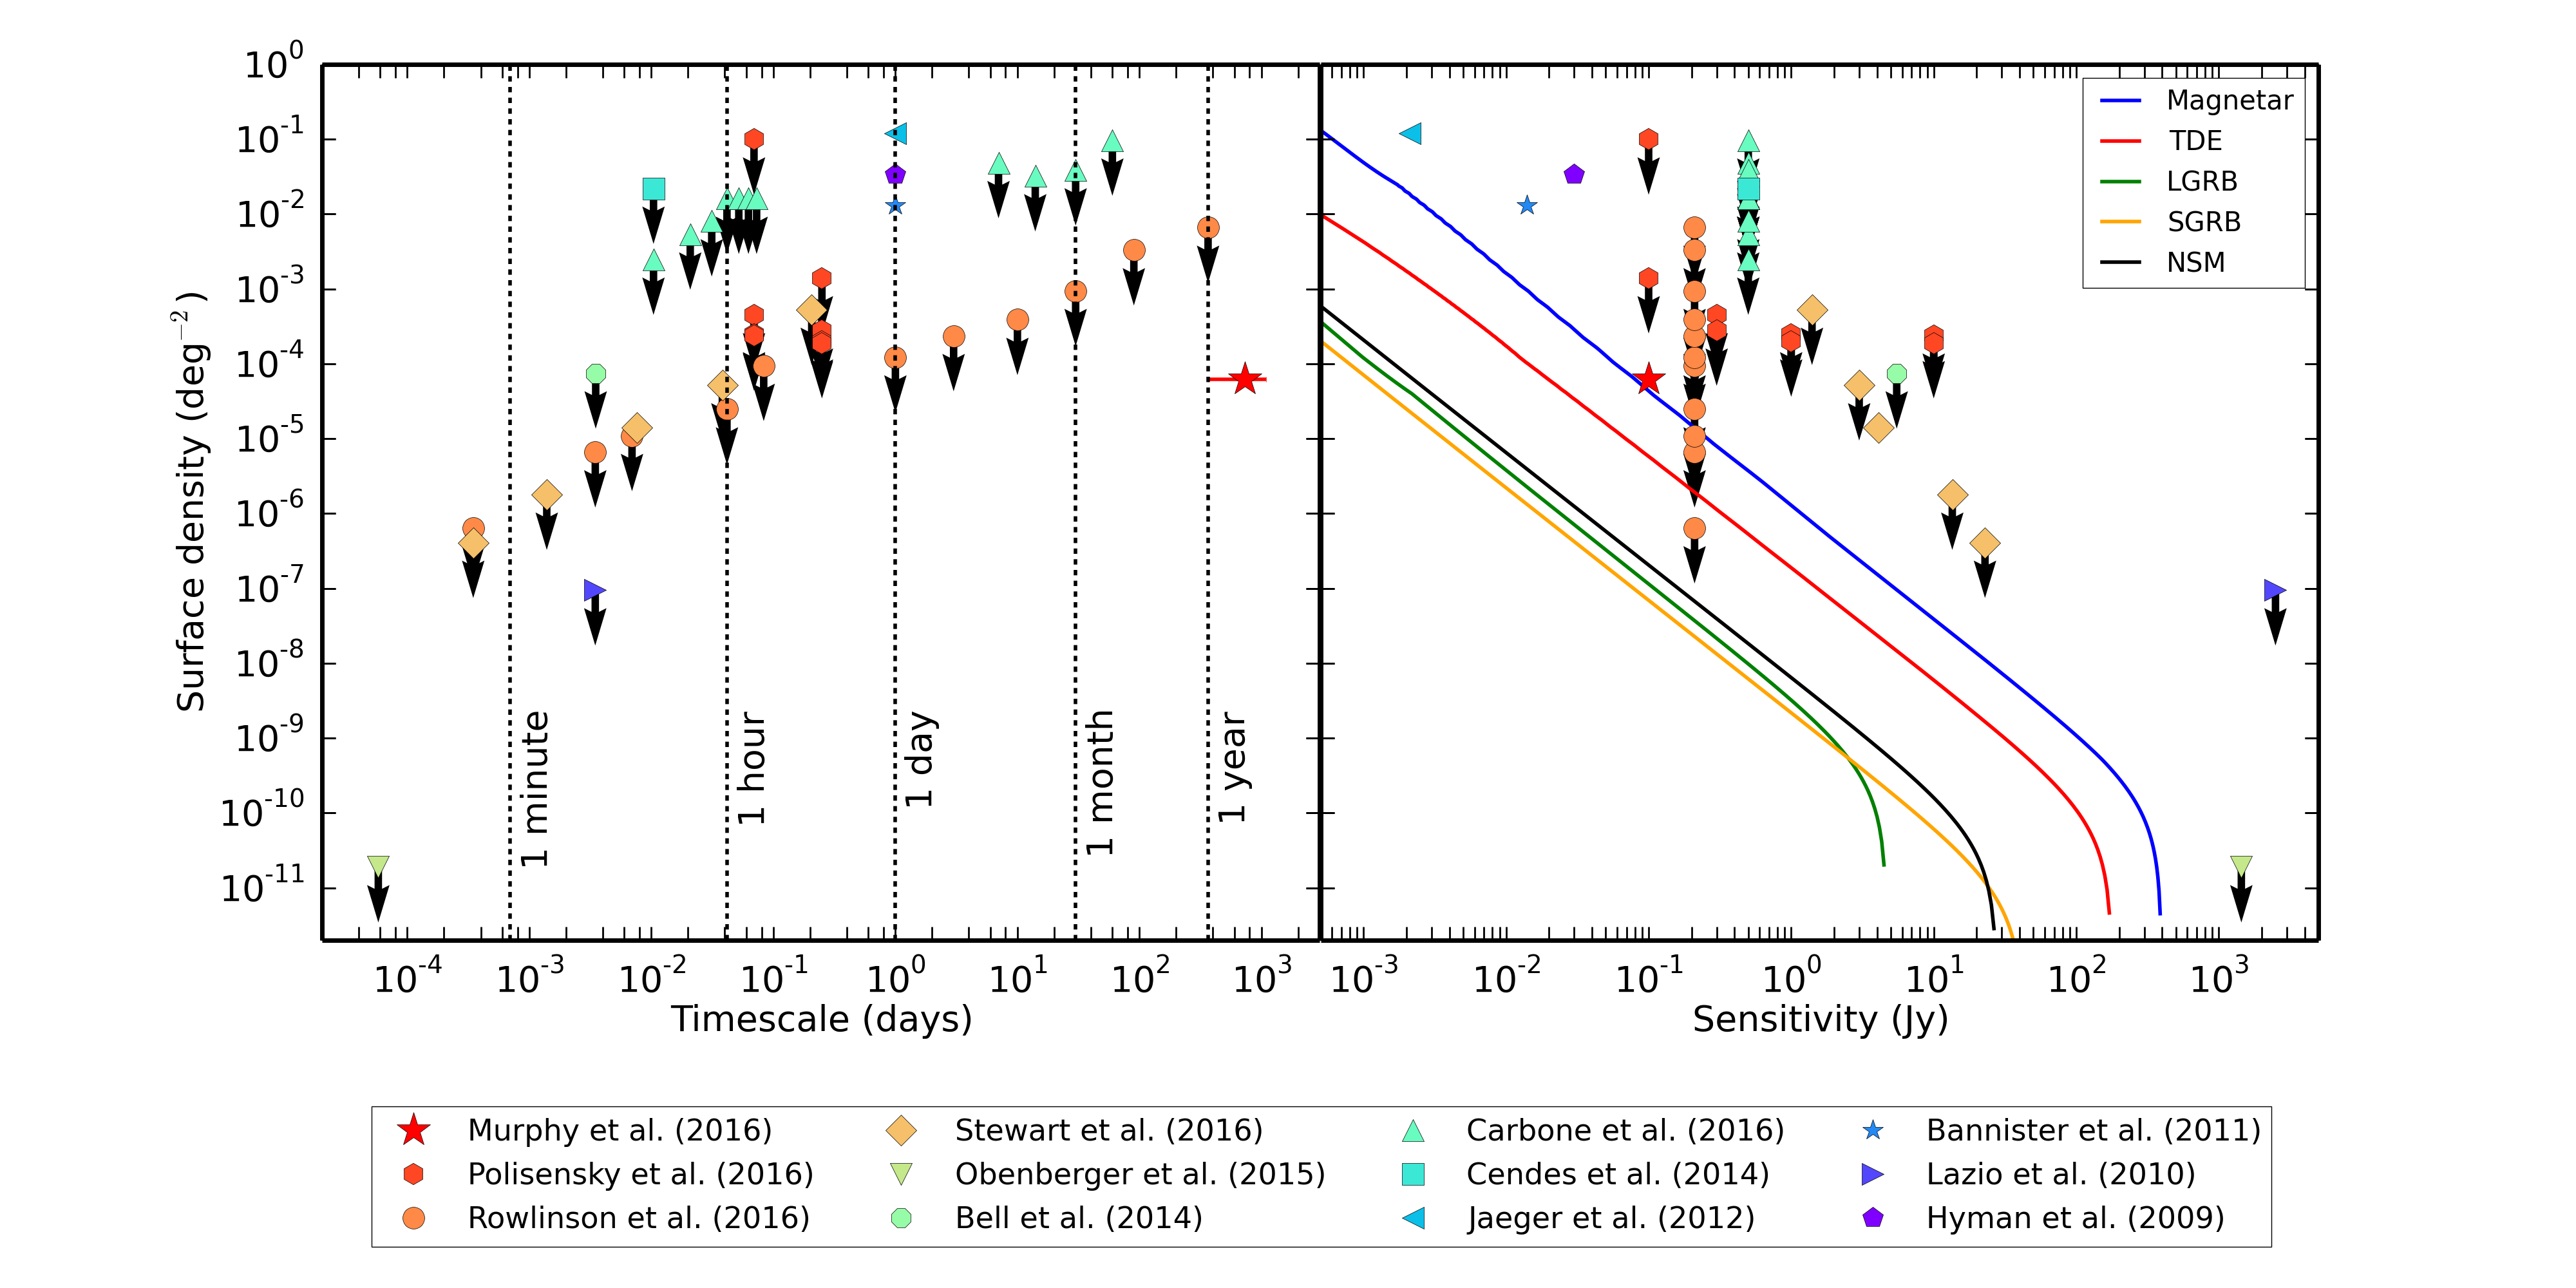
\includegraphics[width=\textwidth]{rates.png}
		\caption{As shown in \cite{2017MNRAS.466.1944M}, various transient searches below 1 GHz have probed a portion of parameter space, but there is much more that can be done. The lines for the various kinds of objects are from \cite{2015ApJ...806..224M}.}
		\label{murphy2017}
	\end{figure}


	\begin{figure}
		\begin{center}
			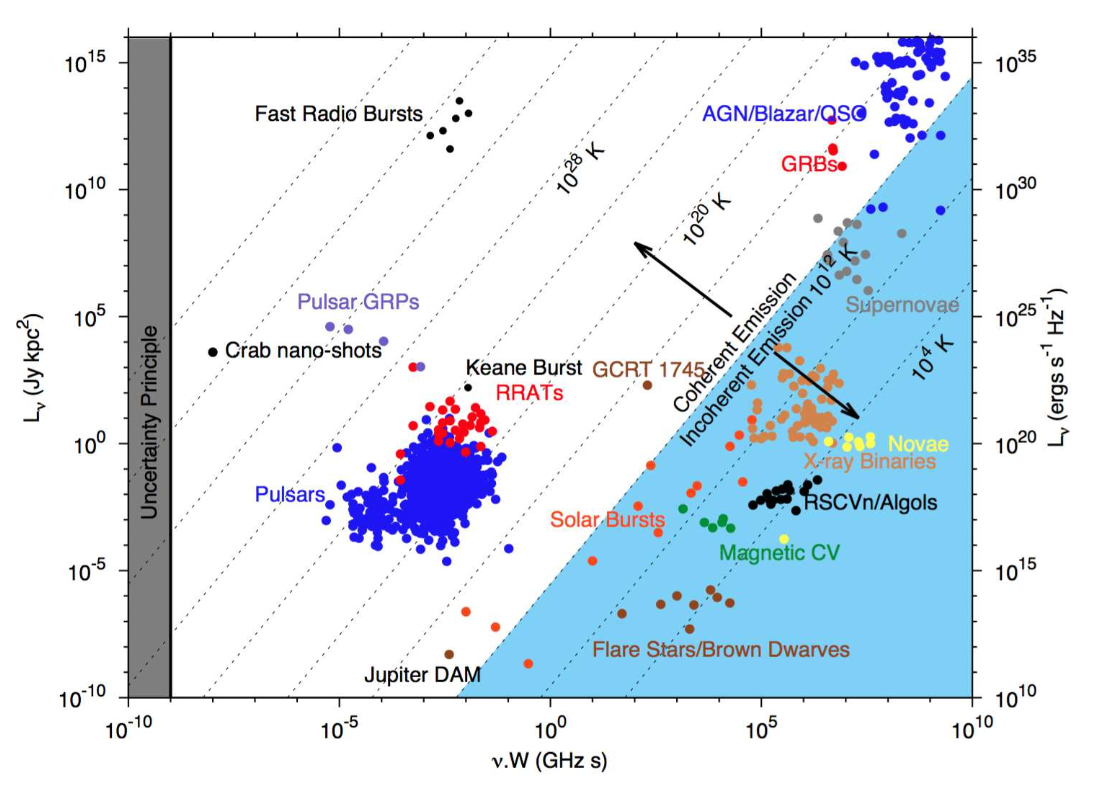
\includegraphics[width=\textwidth]{dario_var_lum.png}
			\caption{From \cite{2015MNRAS.446.3687P}, spectral luminosity plotted against the observing frequency multiplied by pulse width. The diagonal lines represent different brightness temperatures.}
			\label{dario_var_lum}	
		\end{center}
	\end{figure}


\subsubsection{New and Promising Telescopes}
Up until fairly recently, transient searches were only really practical in the optical, X-rays, or gamma-rays. The ability to do transient searches in radio has come with upgrades to existing facilities such as the improved sensitivity and frequency range of the Jansky Very Large Array (VLA or JVLA) \cite{2011ApJ...739L...1P} and the rise of new radio facilities such as the MeerKAT Karoo Area Telescope \cite{2016mks..confE...1J} with its wide field of view and unparalleled sensitivity in its observing bands, the Low Frequency Array (LOFAR) \cite{2013A&A...556A...2V} with excellent sensitivity in low radio frequencies and capabilities for resolving very small objects by using the antennae spanning the European continent, the Murchison Widefield Array (MWA) \cite{2013PASA...30....7T} with its excellent sensitivity at low frequencies and wide field of view, the Australian Square Kilometer Array Precursor (ASKAP) \cite{2014PASA...31...41H} with its wide field of view and excellent survey speed, and other instruments, along with computers advanced enough to process the data. For example, the Square Kilometer Array (SKA) \cite{2009IEEEP..97.1482D}, for which many of the aforementioned telescopes are pathfinders, is expected to need exascale-level computing power and efficiency to operate effectively \cite{doi:10.1177/1094342014549059}. 

The upgraded VLA \cite{2011ApJ...739L...1P} began observing in 2012 and provided a vast improvement over the previous generation. It allowed for increased sensitivity, additional and broader observing frequency bands, and vastly improved correlators and other equipment, allowing for better flagging and finer frequency resolution. Sensitivity increases help a great deal for transient follow-up observations. For instance, for gamma-ray bursts (GRBs), the VLA is used to follow up on detections made in other bands. Observing in the radio can provide a much clearer picture of the physics behind these events, and the upgrade makes that possible for a much larger sample than before (which was sensitivity limited \cite{Chandra_2012}). It also was a valuable resource in following up on the first electromagnetic counterpart to a gravitational wave event, GW170817, an event that was quite remarkable in the amount of new knowledge gained in several areas of physics. The peak flux of this event was at the border of what the old VLA could have observed. After this detection with the VLA, I participated in a collaboration using the VLA to follow up on gravitational wave events. This resulted in an observation for which we obtained upper limits~\citep{2019GCN.26527....1C}. In addition to following up on gravitational waves, I also assisted with a search for a radio counterpart to an extragalactic magnetar~\cite{2021Natur.589..207R}.

MeerKAT \cite{2016mks..confE...1J} is a radio interferometer in South Africa that has recently come online (summer of 2018), will be part of SKA Phase 1, and observes at UHF (544-1087 MHz), L-band (856-1711 MHz), and S-band (1750-3499 MHz). With a field of view of more than a square degree at 1280 MHz, MeerKAT provides one of the best chances to find transients in this observing band. It is also well suited for transient follow-up since it has better sensitivity than the VLA between 1 and 2 GHz. 

In light of the excellent capabilities of MeerKAT, ThunderKAT \cite{2016mks..confE..13W} is a large program on MeerKAT with the goal of studying radio transients. Many important results have come from observations by the ThunderKAT collaboration such as the x-ray binaries in~\citet{2020NatAs...4..697B}, new transient discoveries discovered in commensal transient searches such as in~\citet{2020MNRAS.491..560D} and~\citet{2022MNRAS.513.3482A}, discoveries of variable sources and limits on transient rates such as in~\citet{2022MNRAS.517.2894R} and ~\citet{commensal1}, and many more. The wealth of deep observations taken by MeerKAT ought to be ideal for studying radio transients like never before, perhaps even engaging citizen scientists in new ways as well~\footnote{https://www.zooniverse.org/projects/alex-andersson/bursts-from-space-meerkat/}.

\subsection{Following Up on Transients}
In addition to searching for transients, the radio regime is used to follow up on transient phenomena that have been discovered in the optical, X-rays, or gamma-rays. GRBs and gravitational wave events make for prime examples of transient follow up in the radio and its value to our understanding of high-energy astrophysical phenomena. 

\subsubsection{Gamma-Ray Burst Afterglows}
GRB afterglows were discovered to follow the prompt emission of GRBs in 1997 and the first radio afterglow emission was found for GRB 970508 \cite{1997Natur.389..261F}. GRB afterglows have a distinct synchrotron spectrum with multiple segments and characteristic frequencies \cite{1999ApJ...523..177W, 1998ApJ...497L..17S}. These frequencies correspond to the minimum energy for the electron energy distribution, the synchrotron self-absorption frequency, and the cooling frequency. These characteristic frequencies and the peak flux evolve with a certain time dependence and typically follow the Blandford-McKee solution for a relativistic blast wave at early times \cite{1976PhFl...19.1130B}. The behavior of the spectra can reveal a number of physical properties of the collimated outflow, or jet, produced in the GRB explosion, the emission processes at play, and the environment. Radio follow up is essential for getting a clear picture of the long term behavior since the afterglow is visible in radio long after the optical and X-rays have disappeared, and in some cases, even until the non-relativistic Sedov-Taylor behavior \cite{1959sadm.book.....S, doi:10.1098/rspa.1950.0050} (e.g. GRB 030329 \cite{2008A&A...480...35V}). In particular in the radio, the breaks in the synchrotron spectrum related to the minimum energy of the electron energy distribution and the self absorption are more clearly detectable than in other bands \cite{2014PASA...31....8G}. In addition, the effects of both the forward and reverse shock are visible for a much longer time. The ability to observe the reverse shock can prove valuable for learning more about the properties of the jet itself, since the reverse shock is propagating through it \cite{2014MNRAS.444.3151V, 2013ApJ...776..119L, 2014ApJ...781...37P}. From multi-wavelength observations, in which the radio band plays a crucial role, we can determine physical parameters of the explosion (e.g. the energy), the environment (e.g. the ambient medium density), and the electrons and magnetic fields necessary to produce the synchrotron emission \cite{2014PASA...31....8G}. These parameters can be constrained for both long and short GRBs\footnote{Long GRBs are those which have $T_{90}>2$ seconds, where $T_{90}$ is the time during which 90\% of the gamma-ray counts are detected above background \cite{1993ApJ...413L.101K}.}, where the former is associated with the collapse of a massive star \cite{1998Natur.395..670G, 2003Natur.423..847H, 1993ApJ...405..273W} and the latter with the merger of two compact objects \cite{1989Natur.340..126E, 1992ApJ...395L..83N, 2017PhRvL.119p1101A}. While radio detections of afterglows from long GRBs have been occuring with regularity for some time now, radio detections of afterglows from short GRBs is still quite rare~\citep{2015ApJ...815..102F}. It is still not completely clear why it is so challenging to detect these afterglows in radio, but we will investigate some possible reasons of this in chapter 5.

\subsection{Structure of the Thesis}
In chapter 2 we will demonstrate how we have created accurate transient rate calculations by using Monte-Carlo simulations. In particular, we will show how starting with either a real or simulated observational setup, the simulations code calculates a transient rate as a function of transient duration and peak flux. These simulations allow for simulating a wide variety of scenarios including observations with varying sensitivities and durations, multiple overlapping telescope pointings, and a wide variety of light curve shapes and are easily adaptable to particular science cases.

In chapter 3, we will report on a commensal search in deep observations of short gamma-ray burst fields carried out with the MeerKAT radio telescope in South Africa. These four hour observations of eight different fields span survey lengths of weeks to months. We also carry out transient searches in time slices of the full observations, at timescales of 15 minutes, and 8 seconds. We found 122 variable sources on the long timescales, of which 52 are likely active galactic nuclei, but there are likely also some radio flaring stars. While the variability is intrinsic in at least two cases, most of it is caused by interstellar scintillation. We will also place constraints on transient rates based on state-of-the-art transient simulations codes.

In the following chapter 4, we will report on another commensal transient search of supernovae and short gamma-ray burst fields using methodology established in chapter 3. We search for transients in images with 30 minute integration times finding 12 variable sources. Of these variables, most of them are likely scintillating active galactic nucleii, but one is not consistent with scintillation. We will discuss possible reasons for this variability. Finally we will establish accurate upper limits on the transient rate using transient simulations, establishing upper limits a factor of two lower than the previous search in chapter 3. 

Finally in chapter 5, we will use deep MeerKAT observations of short gamma-ray burst fields to establish upper limits on possible afterglow emission. We then can use these upper limits to place constraints on astrophysical parameters. In particular, we will show that with the full SKA-1 we should be able to determine whether or not the gamma-ray efficiency is significantly lower for short gamma-ray bursts compared to long gamma-ray bursts. In addition, if it is indeed lower, we should expect to start regularly detecting short gamma-ray burst afterglows with SKA-1. Furthermore, we also report the detection of host galaxies associated with these short gamma-ray bursts for a number of cases and calculate the star formation rate, assuming the radio emission is from star formation.


\newpage
\section{Conclusions}
\label{conc}
\subsection{Summary}
Several new radio facilities have a field of view and sensitivity well suited for transient searches. This makes it more important than ever to accurately determine transient rates in radio surveys. Chapter 2 demonstrates how we have done this task by using Monte-Carlo simulations. In particular, the user inputs either a real or simulated observational setup, and the simulations code calculates transient rate as a function of transient duration and peak flux. These simulations allow for simulating a wide variety of scenarios including observations with varying sensitivities and durations, multiple overlapping telescope pointings, and a wide variety of light curve shapes with the user having the ability to easily add more. 

In chapter 3, we present a commensal search in deep observations of short gamma-ray burst fields carried out with the MeerKAT radio telescope in South Africa. These four hour observations of eight different fields span survey lengths of weeks to months. We also carry out transient searches in time slices of the full observations, at timescales of 15 minutes, and 8 seconds. We find 122 variable sources on the long timescales, of which 52 are likely active galactic nuclei, but there are likely also some radio flaring stars. While the variability is intrinsic in at least two cases, most of it is caused by interstellar scintillation. We also placed constraints on transient rates based on state-of-the-art transient simulations codes.

In the following chapter 4, we carry out another commensal transient search of supernovae and short gamma-ray burst fields using methodology established in chapter 3. We search for transients in images with 30 minute integration times finding variable sources. Of these variables, most of them are likely scintillating active galactic nucleii, but one is not consistent with scintillation. We discussed possible reasons for this variability. Finally we calculated accurate upper limits on the transient rate using transient simulations establishing upper limits a factor of two lower than the previous search in chapter 3. 

Finally in chapter 5, we used deep MeerKAT observations of short gamma-ray burst fields to establish upper limits on possible afterglow emission. We used these upper limits to place constraints on astrophysical parameters. In particular, we found that with the full SKA-1 we should be able to determine whether or not the gamma-ray efficiency is significantly lower for short gamma-ray bursts compared to long gamma-ray bursts. In addition, if it is indeed lower, we expect to start regularly detecting short gamma-ray burst afterglows with SKA-1. Furthermore, we also detect the host galaxy associated with these short gamma-ray bursts for a number of cases and calculate the star formation rate, if all the radio emission were from star formation. 
\subsection{Future Work}
\subsubsection{Continued Commensal Searches} 
Continuing to conduct commensal searches is an important way to continue to place tighter and tighter limits on the transient population in radio. By continuing to search for transients in the 8 second images that come from the MeerKAT radio telescope, we can probe a rarely examined part of parameter space and possibly start placing limits on the FRB limits from image searches alone. 

Additionally, given the low cost of conducting transient searches on longer timescales, continuing to carry out transient searches on these timescales, using the software and methodologies established in chapters 3 and 4, provides easy opportunities to find interesting transients. Along with potential transients, these surveys will provide deeper and deeper limits on transient rates, which may eventually allow for calculating rates that accurate to specific kinds of sources.

\subsubsection{Improved Transient Simulations}
Even though the transient rate simulations presented in chapter 2 are much more accurate than other methods, they still have room for improvement. Improvements to the way in which the transient population is simulated will provide a deeper understanding of how the transient rate changes over parameter space. Additionally, spatially dependent transient population simulations may help improve transient rate calculations and help with better understanding galactic versus extragalactic transients. Another important improvement will be testing the light curves that are included with the simulations to ensure that the simulated light curves are producing results that match with real light curves. 
\newpage
\section{References}
{\def\section*#1{}
\singlespacing
\bibliographystyle{aasjournal}
\bibliography{bibliography}
}
\newpage
\newgeometry{top=1in, bottom=1in, left=1.25in, right=1.25in}



\doublespacing
\appendix


\section{Appendix}\label{appendixlabel}
%Figure \ref{fig:snr_pipeline} is an example figure.
%\begin{figure}[htb!]
%    \centering
%    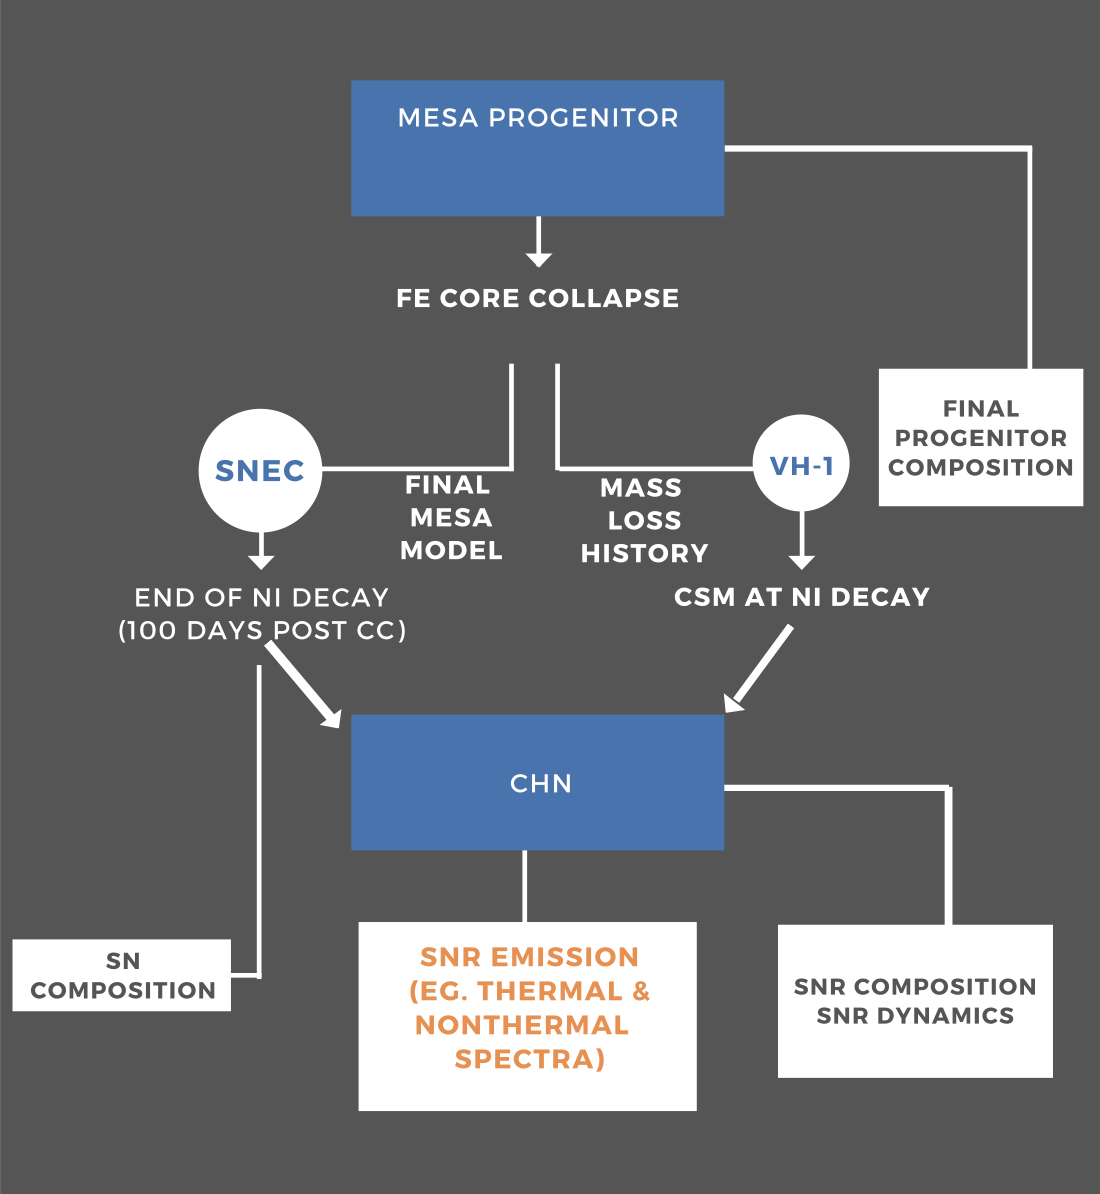
\includegraphics[width=\textwidth]{SNR_pipeline.png}
%    \caption{Example figure}
%    \label{fig:snr_pipeline}
%\end{figure}


\end{document}

